% Created 2023-08-30 Wed 10:10
% Intended LaTeX compiler: pdflatex
\documentclass[11pt]{article}
\usepackage[utf8]{inputenc}
\usepackage[T1]{fontenc}
\usepackage{graphicx}
\usepackage{longtable}
\usepackage{wrapfig}
\usepackage{rotating}
\usepackage[normalem]{ulem}
\usepackage{amsmath}
\usepackage{amssymb}
\usepackage{capt-of}
\usepackage{hyperref}
\usepackage{minted}
\usepackage[a4paper]{geometry}
\usepackage{mathtools}
\usemintedstyle{mathematica}
\author{Alexander Huss}
\date{\today}
\title{Transverse Momentum Resummation}
\hypersetup{
 pdfauthor={Alexander Huss},
 pdftitle={Transverse Momentum Resummation},
 pdfkeywords={},
 pdfsubject={},
 pdfcreator={Emacs 29.1 (Org mode 9.7)}, 
 pdflang={English}}
\begin{document}

\maketitle
\tableofcontents



\section{Introduction}
\label{sec:org3533e17}
In the lectures we have seen a brief overview of the \(q_T\) resummation formalism for the Drell-Yan process.
We will have a closer look at the main results here and highlight some features.

\section{\(q_T\) resummation}
\label{sec:org5242176}
In the leading double-logarithmic approximation, we have found the following result in impact parameter space
\begin{align}
\label{eq:b-space}
  \frac{1}{\sigma_0}\,\frac{\mathrm{d}\sigma}{\mathrm{d}q_T^2}
  &=
  \int_0^\infty\mathrm{d}b \, \frac{b}{2} \, J_0(q_T b) \,
  \exp\Big[
    -\frac{\alpha_s}{2\pi}\, C_F \, \ln^2(Q^2 b^2)
  \Big]
  \,,
\end{align}
where we have completely ignored effects from sub-leading logarithms, the running of the strong coupling, and parton distributions functions.
Nonetheless, this simple formula already allows us to inspect some important features of \(q_T\) resummation, which we will inspect in the following.


\section{Implementation}
\label{sec:org394c021}
We start with a simple implementation of the above formula.

\subsection{Python}
\label{sec:org2e3e44d}
The integral is a bit nasty because of the oscillating behaviour of the Bessel funtion \(J_0\) so we need to adjust the \texttt{scipy.integrate} settings a little bit to reach a desired accuracy.
Despite that, the implementation is straightforward:
\begin{minted}[frame=lines,fontsize=\scriptsize]{python}
#!/usr/bin/env python
import sys
from math import pi, exp, log, log10, ceil, floor
from scipy.special import jv  # Bessel function of the 1st kind
from scipy.integrate import quad
import numpy as np

alpha_s: float = 0.118


def res_integrand(b: float, QT: float, Q: float, CX: float) -> float:
    b0: float = 2. * exp(-0.57721566490153286061)
    # blim: float = 5.  # should be > 1/Lambda_QCD ~ 5
    # bs2: float = b**2 * blim**2 / (b**2 + blim**2)
    # return (b / 2.) * jv(0, b * QT) * exp(
    #     -alpha_s / (2. * pi) * CX * log(Q**2 * bs2 / b0**2 + 1.)**2)
    return (b / 2.) * jv(0, b * QT) * exp(
        -alpha_s / (2. * pi) * CX * log(Q**2 * b**2)**2)


if __name__ == "__main__":
    if len(sys.argv) < 3:
        raise RuntimeError("I expect at least two arguments:  Q [g|q]")
    Q = float(sys.argv[1])  # the hard scale
    pow_low = -3
    pow_upp = ceil(log10(Q/2.)) # floor(log10(Q))
    if sys.argv[2].lower() == "q":
        CX = 4. / 3.
    elif sys.argv[2].lower() == "g":
        CX = 3.
    else:
        raise RuntimeError("unrecognised parton: {}".format(sys.argv[2]))

    if len(sys.argv) >= 4:
        alpha_s = float(sys.argv[3])

    if len(sys.argv) >= 5:
        nsteps = int(sys.argv[4])
    else:
        nsteps = 51

    # print("# qt dSigQT2_val dSigQT2_err")
    for qt in np.logspace(pow_low, pow_upp, nsteps):
        val, err = quad(res_integrand,
                        0.,
                        np.inf,
                        args=(qt, Q, CX),
                        epsabs=0.,
                        epsrel=1e-4,
                        limit=100000)
        print("{}  {} {}".format(qt, val, err))
\end{minted}

And we can generate some data files for Drell-Yan and Higgs production where in the latter we simply swap out the colour charge \(C_F \to C_A\) for the gluon-fusion process.
\begin{minted}[frame=lines,fontsize=\scriptsize]{shell}
python main.py  91 q > data_dy.dat
python main.py 125 g > data_h.dat
\end{minted}

\subsection{Mathematica}
\label{sec:org34b8f81}
To cross-check the numerics, we can use a simple Mathematica implementation
\begin{minted}[frame=lines,fontsize=\scriptsize]{wolfram}
dSigQT2[qt_] := Module[{cf = 4/3, as = 0.118, q = 91},
  NIntegrate[b/2 BesselJ[0, b*qt] Exp[-(as/(2 Pi)) cf Log[q^2 b^2]^2], {b, 0, Infinity}]
]
datQT2 = Table[{qt, dSigQT2[qt]}, {qt, 10^Range[-4, 2, 0.1]}]
Export["mma_dy.dat", datQT2, "Table", "FieldSeparators" -> " "]
\end{minted}


\section{Playground}
\label{sec:org2b3ed46}

\subsection{Low-\(q_T^2\) behaviour}
\label{sec:orgce81e6a}
Let us have a look at the analytic expression for \(\mathrm{d}\sigma/\mathrm{d}q_T^2\) in the leading double-logarithmic approximation in momentum space.
\begin{align}
  \frac{1}{\sigma_0}\,\frac{\mathrm{d}\sigma}{\mathrm{d}q_T^2}
  &=
  \frac{\alpha_s}{\pi}\, C_F \, \frac{\ln(Q^2 q_T^2)}{q_T^2}
  \exp\Big[
    -\frac{\alpha_s}{2\pi}\, C_F \, \ln^2(Q^2 q_T^2)
  \Big]
  \,.
\end{align}
This expression can be obtained from Eq. \eqref{eq:b-space} by systematically expanding the Fourier transform or alternatively by naively resumming the emissions \emph{without} the transverse momentum conservation constraint.

We can compare this expression with the numerically evaluated b-space formula from above:
\begin{center}
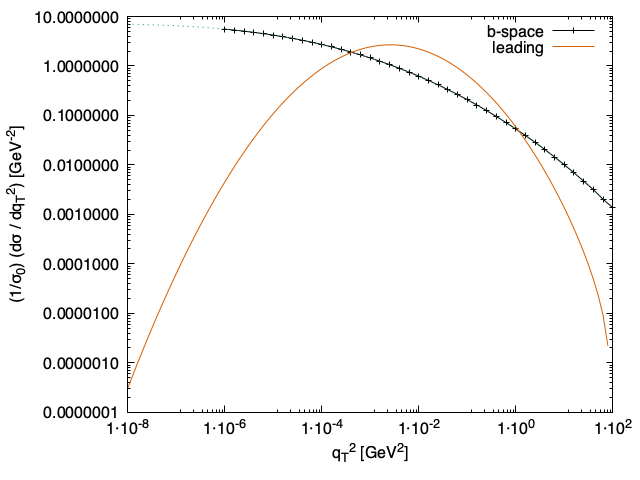
\includegraphics[width=.9\linewidth]{plot_QT2.png}
\end{center}

We notice that the leading expression shows a strikingly different behaviour in the small \(q_T^2\) limit compared to the b-space formula.
The physical interpretation is quite clear: the leading term corresponds to restricting \emph{all} gluon emissions to have \(k_T\) below the gauge-boson transverse momentum \(q_T\).
This gives a suppression at low \(q_T\) that is stronger than any power and as a consequence, the sub-leading effect suddenly becomes the leading one.
In this situation, the small-\(q_T\) region is not restricted to only soft gluon emissions but instead by multiple gluon emissions that can individually have \(k_T > q_T\) but they \emph{balance out} in the azimuthal plane.
By formulating the resummation in impact parameter space, this feature is automatically incorporated in the prediction.

This non-vanishing intercept in \(\mathrm{d}\sigma/\mathrm{d}q_T^2\) for \(q_T\to0\) is a very important feature of transverse momentum resummation.
In fact, we can compute what this intercept is
\begin{align}
  \frac{1}{\sigma_0}\,\frac{\mathrm{d}\sigma}{\mathrm{d}q_T^2} \biggr\rvert_{q_T=0}
  &=
  \frac{\pi}{2 Q^2}\;\frac{\mathrm{e}^{\frac{\pi}{2\alpha_s C_F}}}{\sqrt{2\alpha_s C_F}}
  \,.
\end{align}

We have also superimposed a dotted line obtained from the Mathematica implementation, which is in good agreement so numerics appear to be under good control in the relevant regions.
At high \(q_T\), the oscillations become very severe rendering the pPython predictions less reliable (with larger integration errors).

\subsection{Transverse Momentum Distributioins}
\label{sec:orga755d2d}
We now look at the transverse momentum distribution, which we simply get by
\begin{align}
  \frac{\mathrm{d}\sigma}{\mathrm{d}q_T}
  &=
  2 q_T \; \frac{\mathrm{d}\sigma}{\mathrm{d}q_T^2}
  \,,
\end{align}
from the data we generated.
We can contrast it to the divegent behaviour
\begin{align}
  \frac{1}{\sigma_0}\,\frac{\mathrm{d}\sigma}{\mathrm{d}q_T^2}
  &=
  \frac{\alpha_s}{\pi}\, C_F \, \frac{\ln(Q^2 q_T^2)}{q_T^2}
\end{align}
of an NLO fixed-order prediction (dashed lines).
\begin{center}
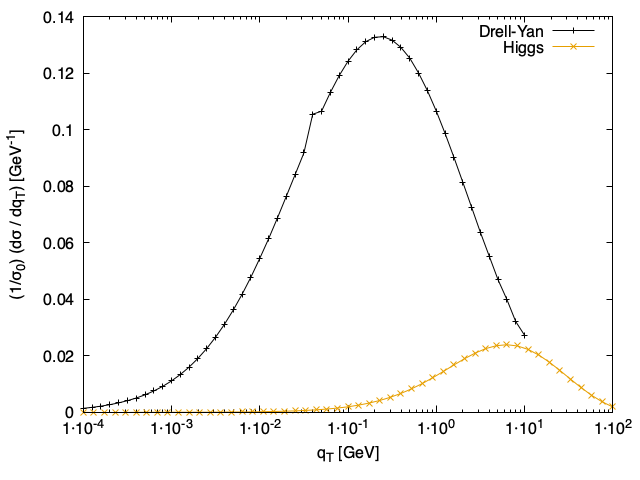
\includegraphics[width=.9\linewidth]{plot_dy.png}
\end{center}
Note that \(\mathrm{d}\sigma/\mathrm{d}q_T\) vanishes for \(q_T\to0\), however, the \(q_T^2\) behaviour we discussed in the previous section makes it a power-like suppression rather than an exponential one we would get from the naive leading behaviour.
The resummation tames the divergent fixed-order behaviour and the turn-around point is also often called the ``Sudakov peak''.
We see that due to the larger colour charge in the gluon-induced Higgs process (\(C_A = 3 > \tfrac{4}{3} = C_F\)), the localtion of the Sudakov peak is further to the right in that case.
\end{document}